\documentclass{article}
\usepackage{graphicx}
\usepackage{tabularx}
\usepackage{fancyhdr}
\usepackage{cite}
\usepackage{hyperref}
\usepackage{lipsum}
\usepackage{xcolor}
\usepackage{colortbl}

\pagestyle{fancy}
\setlength{\footskip}{60pt}
\vspace{-2cm}
\fancyfoot{\rule{0.5\linewidth}{1pt}}

\fancyfoot[L]{{
\includegraphics[scale=0.10]{logo.png}}}

\definecolor{lightgreen}{rgb}{0.56, 0.93, 0.56}

\begin{document}


\begin{center}

\includegraphics[scale=0.2]{logo.png}
\end{center}

\vspace{0.5cm}

\begin{center}

 Group 201: Amir Ghari, Heejin Kim, Aleskanteri Merilainen, Eiaki Morooka \\

\vspace{0.5cm}

{\Huge \textcolor{red}{Hardware 1 Project Plan}} \\


\vspace{0.5cm}

{\Large \textbf{Project plan}} \\


\end{center}

\vspace{1cm}

\begin{center}

{\Large }



\begin{tabular}{l}
 First year hardware project \\
 School of ICT\\
 Metropolia University of Applied Sciences  \\
 \today \, (v0.2)
\end{tabular}
\end{center}

\newpage

\begin{abstract}
Group 201, a team of 1st-year students at Metropolia University of Applied Sciences, School of ICT, is developing a heart rate detection and analysis system using photoplethysmography (PPG) technology. The project's objectives include creating a user-friendly device for measuring heart rate and heart rate variability, connecting to Kubios Cloud HRV analysis service, and displaying estimated stress and recovery status indexes. The team plans to use various communication tools and methods to ensure good group communication and proper version control of project-related materials. The project is part of a course curriculum and scheduled to be completed by May 5th.
\end{abstract}





\vspace{1cm}

\begin{table}[h]
\centering
\begin{tabular}{|p{1cm}|p{5cm}|c|p{3.5cm}|}
\hline
\textbf{Ver} & \textbf{Description} & \textbf{Date} & \textbf{Author(s)} \\ \hline
1.0 & Created structure for the project plan. Added instructions for what should be included in the various parts of the document.   & 31.1.2023 & Saana Vallius \\ \hline
1.1 & Review meeting. Notes are shown with yellow.  & 6.2.2023 & Joseph Hotckiss,  Keijo Lanskinnas, Saana Vallius, Miguel Cheneuer, Sakari Lukkarinen \\ \hline
1.2 & Updated commented parts according to what was decided in the review meeting. Changed the name of the document. & 7.3.2023 & Saana Vallius \\ \hline
1.3 &  Removed mentions of adding teachers to Teams workspace. & 9.3.2023 & Saana Vallius \\ \hline
1.4 &  Details added to Introduction, Project Description, Communication, Version Control, Schedule, and Goals based on our group's specific needs.  & 11.3.2023 & Amir Ghari, Heejin Kim, Aleksi Merilainen, Eiaki Morooka \\ \hline
 &  &  &  \\ \hline
 &  &  &  \\ \hline
\end{tabular}
\caption{Version history}
\label{table:version-history}
\end{table}

\begin{center}
\textbf{\large Keywords:}
\end{center}
\begin{bf}
\begin{center}
\fbox{
\parbox{0.8\textwidth}{
 Heart Monitor \\ Raspberry Pi Pico \\ Game
}
}
\end{center}
\end{bf}

\newpage

\tableofcontents

\newpage

\section{Introduction}

This document is a project plan that details the development of a heart rate detection and analysis system by Group 201, a team of 1st year students at Metropolia University of Applied Sciences, School of ICT. The system will use photoplethysmography (PPG) technology to measure blood volume changes in the microvascular bed of tissue to determine a user's heart rate and heart rate variability (HRV). The plan covers the project's objectives, timeline, team roles, communication methods, and the hardware components used to build the system.



The project aims to create a device that can be used in home or office environments by end-users or health and wellbeing professionals, such as physiotherapists, nurses, or medical doctors. The project is part of a course curriculum that involves utilizing the Raspberry Pi Pico microcontroller board and other components to develop a proof-of-concept for the recovery and stress meter.



The development of the heart rate detection and analysis system focuses on five main objectives, including developing a heart rate detection algorithm, calculating HRV analysis, enabling the device to send, store, and read HRV data, building a connection to Kubios Cloud HRV analysis service, and developing a feature that shows estimated stress and recovery status indexes on the device.



The project is scheduled to be completed by May 5th, following a timeline consisting of five stages, including Discover, First stage, Second stage, Third stage, and Final release. The team plans to cultivate various skills during this project, including utilizing the knowledge gained in Hardware 1 and Network classes, understanding programming for implementing hardware products by using Micropython, improving IT documentation writing skills, and improving communication skills. The team plans to use various communication tools and methods, including in-person and online meetings, Discord, GitLab, and Microsoft Teams, to ensure good group communication and proper version control of project-related materials.



\section{Project Description}

The project aims to create a heart rate detection and analysis system that utilizes photoplethysmography (PPG) technology to measure blood volume changes in the microvascular bed of tissue. By detecting changes in blood volume, the system can determine a user's heart rate and heart rate variability (HRV).



To achieve this goal, the project will focus on five main objectives. First, the team will develop a heart rate detection algorithm that can work locally on the device. This will allow the system to provide accurate heart rate measurements without requiring an internet connection.



Second, the team will work on calculating HRV analysis using the data collected by the PPG sensor. HRV is a measure of the variation in time between each heartbeat, and it can provide valuable information about a user's health and stress levels.



Third, the team will enable the device to send, store, and read HRV data to/from a server. This will allow users to access their data from different devices and locations and enable health and wellbeing professionals to remotely monitor their clients' HRV data.



Fourth, the team will build a connection to Kubios Cloud HRV analysis service. This service provides more detailed HRV analysis and can help users and professionals to better understand their HRV data.



Finally, the team will develop a feature that shows estimated stress and recovery status indexes on the device. This will enable users to monitor their stress levels and recovery status in real-time and adjust their lifestyle accordingly.


The device is intended for use in home or office environments and can be used by end-users or health and wellbeing professionals such as physiotherapists, nurses, or medical doctors. The Raspberry Pi Pico microcontroller board and other components will be used to develop a proof-of-concept for the recovery and stress meter. The Raspberry Pi products are extensively supported by the manufacturers and by the user community, making them a suitable choice for this project.


\begin{figure*}[h]
  \centering
  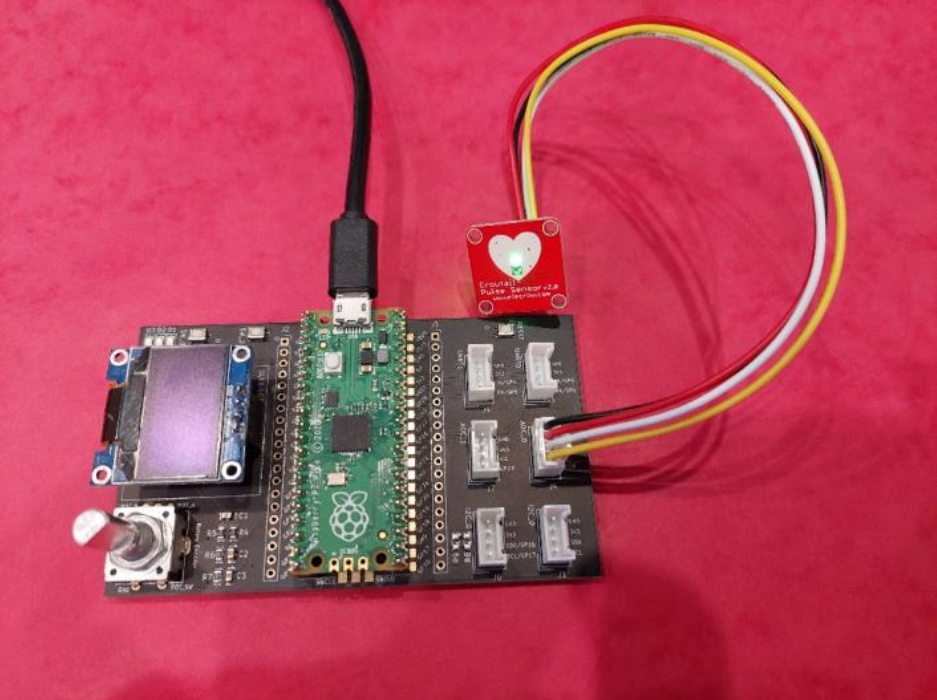
\includegraphics[width=0.7\textwidth]{raspi_heart.png}
  \caption{ Current Raspberry pi pico and its accessories.}
  \label{raspi}
\end{figure*}



\subsection{Hardware}

To develop the heart rate detection and analysis system, the main hardware component being used is the Raspberry Pi Pico, which is a versatile microcontroller board designed for IoT (Internet of Things) devices. The board is small and adaptable to a wide range of applications in home, hobby, education, and industry. It has a rich set of peripherals, including SPI, I2C, and programmable I/O state machines for custom peripheral support. For this project, the board is programmable using MicroPython.



Additionally, there is a wireless version of the board, Raspberry Pi Pico W, which includes a certified wireless LAN module.



The development board used in the project includes a rotary switch and knob, a 128x64 OLED display, 3 LEDs (Light emitting diodes), and two of the three micro buttons for interacting with the board. The board is connected to a laptop or desktop via USB cable, and it includes 4-pin Grove-connectors for connecting serial communication devices such as I2C sensors or analog input sensors. The optical heart rate sensor is connected to one of the Grove-connectors and Pico’s ADC\_0 pin.



Overall, the Raspberry Pi Pico board and associated components provide a flexible and customizable platform for developing the heart rate detection and analysis system. A full list of the components used in the proof-of-concept product is provided in Table 1. An figure of the device is in figure \ref{raspi}, and a block diagram is in figure \ref{diagram}.


\begin{table}[h]
\centering
\begin{tabular}{|p{2cm}|p{5.5cm}|p{4cm}|}
\hline
\textbf{Components} & \textbf{Description} & \textbf{More Info} \\ \hline
Raspberry Pi Pico & Dual-core ARM processor microcontroller having 246 kB SRAM and 2 MB on-board Flash. It also includes 2.4 GHz wireless LAN and 26 multifunction GPIO pins.    & \href{https://www.raspberrypi.com/products/raspberry-pi-pico/}{Raspberry Pi Pico series – Raspberry Pi }    \\ \hline
Crowtail Pulse Sensor v2.0   & Optical heart rate sensor having LED (Light Emitting Diode), photodiode, analog amplifier, and analog signal output. Operating voltage 3-5 V  &  \href{https://www.elecrow.com/crowtail-pulse-sensor-p-1673.html}{Crowtail- Pulse Sensor 2.0 (elecrow.com)}   \\ \hline
OLED display   & SSD1306 compatible 128x64 monochrome organic LED-display. Communicates with I2C or UART-protocol.    & \href{https://docs.micropython.org/en/latest/esp8266/tutorial/ssd1306.html}{Sensors Modules SSD1306 Oled Display | Sensors Modules }

Using a SSD1306 OLED display — MicroPython latest documentation    \\ \hline
Protoboard   & Passive protoboard specially designed for this project to help connect the other components to the Raspberry Pi Pico.   & Joseph Hotchkiss, Project Engineer, Metropolia UAS   \\ \hline
Rotary knob  & Digital rotary knob with push button.    & Joseph Hotchkiss, Project Engineer, Metropolia UAS   \\ \hline
\end{tabular}
\caption{Components}
\label{table:version-history}
\end{table}



\begin{figure*}[h]
  \centering
  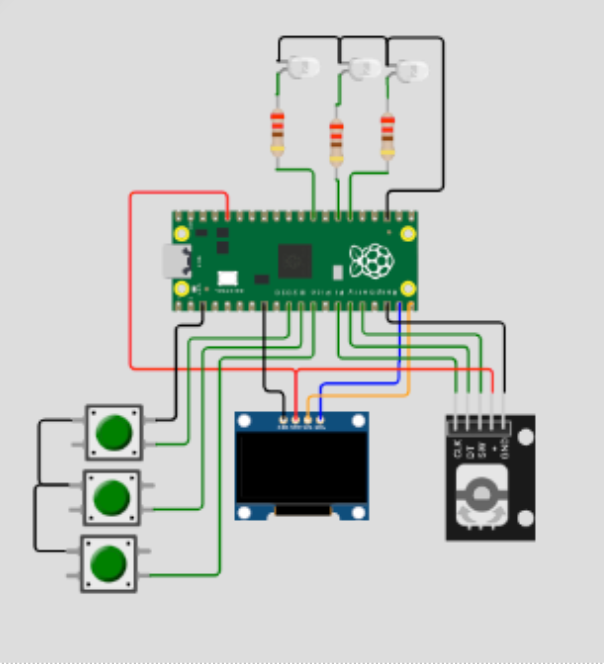
\includegraphics[width=0.7\textwidth]{project_diagram.png}
  \caption{Block diagram of the device}
  \label{diagram}
\end{figure*}


\section{Communication}
Good group communication will be key to a successful project. Therefore, Group201 will communicate using a variety of methods and communication technology tools.

Primarily, the group will meet in-person and online. During the meetings, we share progress, discuss what the next tasks should be, distribute new tasks, and create a schedule for the next meeting. After each meeting, the group creates 'Meeting Notes' to help group members understand and review the discussions that took place. These notes are used to guide the members’ independent work and frame the discussion for the following meeting.

For quick communication, the group uses Discord. A group was created where members share status updates and ask questions or request help from each other.

A GitLab repository is used to efficiently manage, store, and update the project’s code.

A Microsoft Teams workspace provides the group with a work environment where all project-related Word and Excel documents, including the 'Project Plan Template' and 'Project Timetable and Schedule (GANTT) Template,' are stored and updated. Teams also allow group members to comment on each other’s work and to work more collaboratively. Additionally, Meeting notes are stored in the Microsoft Teams workspace in Word document format.

\section{Version Control}
To ensure proper version control of the project code, we have created a private repository in Metropolia GitLab (\href{https://gitlab.metropolia.fi/group201/heart-rate-monitor}{https://gitlab.metropolia.fi/group201/heart-rate-monitor}). This enables us to manage and track the changes made to our project code effectively. By using a version control system, we can easily revert to previous versions if needed, collaborate on the code with other team members, and keep track of who made what changes. In addition, we have included a link to our GitLab repository in our project plan so that it is easily accessible to all project members. We have also added our project teacher as a co-operator to ensure that they can keep track of the progress of our code.



For other project-related materials, we have opted to store everything in our Microsoft Teams workspace. We have created subdirectories as needed to keep everything organized, including one for project-related information and material given to us by our teachers, another for useful reference material we find useful in our project, and a third for our own documents such as project plan, schedule, meeting notes, and project report. By storing everything in one place, we can easily access and share documents with other team members, and our project teacher can also easily monitor our progress.

To keep track of the version control of our own documents, we have produced a naming convention that includes the version number in the file name, such as "main\_v01.py". We also keep a changelog or version history document that tracks changes made to each document, including the date of the change, who made the change, and a brief description of the change. By doing so, we can easily keep track of changes made to documents and avoid confusion or errors. Overall, these practices ensure that our project is well-organized, and all team members can easily access and manage project-related materials.

\section{Schedule}

This project has a timeline consisting of five stages, namely Discover, First stage, Second stage, Third stage, and Final release.

The Discover stage is where the project requirements are understood, and plans are established. It will take place from January 9th to March 12th.

During the First stage, specific project details will be determined, and the devices will be configured and tested. This stage is expected to be completed by early April.

In the Second stage, the project content will be modified and updated based on the improvements identified in the First stage. This stage is expected to take place from early to mid-April.

The Third stage is the final stage where the hardware product plan will be modified, reconfigured, and tested through the attempts made in the First and Second stages. This process is expected from mid-April to the end of April.

Finally, after going through these stages, the product will be released on May 5th with the Final release. The detailed schedule is subject to change and can be confirmed at the link provided below.

\href{https://teams.microsoft.com/\_#/apps/1c256a65-83a6-4b5c-9ccf-78f8afb6f1e8/sections/MyNotebook }{link to project timeline}


\href{https://users.metropolia.fi/~aleksame/Group\%20Project/ }{https://users.metropolia.fi/~aleksame/Group\%20Project/}



\section{Goals}
Group201 aims to cultivate the following skills during this project:



First, we plan to utilize the knowledge gained in Hardware 1 to the fullest to produce the intended heart rate detection and analysis system. Based on the knowledge gained in the Network class, we plan to set up internet connections in real-world environments and utilize them for the operation of the product. We also hope to become more familiar with the command-line interface in Linux, which will help us to become more proficient in the emulation process. In addition, through the Hardware 2 course, we plan to understand programming for implementing hardware products by using micropython.



Secondly, as IT majors, we hope to become familiar with the types of documentation suitable for the IT field. By writing various documents, we expect to learn the writing techniques for each document type.



Lastly, since teamwork is a crucial aspect of IT projects, we hope to improve our communication skills and find effective communication methods while working as a team.



Through the cultivation of these skills, we expect to achieve high-quality project results and receive full grades. To achieve this successful project performance, Group201 plans to go through the following plans.



Firstly, we plan to periodically assign related tasks to each group member. Through regular task allocation and performance, we can quickly identify any shortcomings and, if necessary, seek the help of teachers to improve our skills.



Also, to improve our IT documentation writing skills, we plan to update our documents whenever there are updates and use the memo function to leave feedback on each other's documents.



This will enable us to complete more refined and professional documentation. Memos and feedback not only help with documentation, but also aid in communication among team members. Records left during the project will help all members of the team understand the progress of the project and identify each other's communication styles to make communication between team members easier.


\end{document}
